%---------------------------------------------------------------
\chapter{Introduction}
%---------------------------------------------------------------

%--------------------------------
\section{Objectives of the thesis}
%--------------------------------

%The research part of the thesis will describe what is a \gls{puf} and what are the uses of this technology, focusing mainly on \gls{sram} based \glspl{puf}. Furthermore, the parameters used to evaluate performance of \glspl{puf} will be defined.

%The main objective of the practical part of this thesis is to analyze the possibility of implementing a \gls{sram} based \gls{puf} on the ESP32 family of microcontrollers. This means finding a suitable mechanism of \gls{sram} power control and establishing a way to gather \gls{puf} response data reliably. Next, stability and uniqueness of the obtained \gls{puf} data using the defined parameters will be evaluated. An analysis of the \gls{sram} data depending on different operating temperature and power-off time will be performed as well.

%The next goal will be to implement a simple \gls{sram} based \gls{puf} based on the knowledge gained in the previous experiments. Several different models of devices from the ESP32 family will be used to test the function and performance of the resulting \gls{puf} implementation.

\section{Structure of the thesis}

%---------------------------------------------------------------
\chapter{Physical unclonable functions}
%---------------------------------------------------------------

%--------------------------------
\section{PUF description}
%--------------------------------

As \glspl{puf} are the main subject of this thesis, it is important to provide a thorough explanation of what a \gls{puf} is, what types and classes exist and what are
the applications of this technology.

Since more and more types of \glspl{puf} are being invented, it turns out that creating a generalizable description is not a straightforward task. A dictionary definition of a \gls{puf} could be expressed as: \say{a PUF is an expression of an inherent and unclonable instance-specific feature of a physical object}. One can imagine a \gls{puf} being an object's fingerprint in a comparable way to how humans have their own fingerprints.\cite{Maes2013}

The first concept of \gls{puf} was proposed by Pappu in 2001. He used the term \gls{powf}, which he described as a function operating on a physical system that could be easily computed but not easily inverted.\cite{Pappu2001} The first mention of the term \gls{puf} was by Gassend et al.\ in 2002. He talks about \glspl{prf} and a \gls{puf} implementation using \glspl{fpga}.\cite{Gassend2002}

As \gls{puf} is a function, it has inputs and outputs. However, it is not a function in a true mathematical way. It could be described as a procedure performed on a particular device. Its inputs consist of a challenge and a physical state of the device. Given the input, the \gls{puf} produces an output (called a response). Together, they form challenge-response pairs.   

A hugely important property of \glspl{puf} is unclonability. It is achieved by the physical state of the device which acts as the input to the function and influences the responses produced by the \gls{puf}. The concrete details of the physical state used is what distinguishes different \gls{puf} implementations. These physical properties could be for example propagation delay in the chip circuit or bias of uninitialized memory cells to 1 or 0 state. The latter is a basis for \gls{sram} \gls{puf}, which is a topic of this thesis. These properties are fundamentally random since they are created by uncontrollable physical processes during manufacturing. This makes them physically unclonable.

Since the physical state of the device can change with time and environment (for example temperature or input voltage variations), the challenge-response pairs can change as well. The requirement is, that for the same challenge, the responses should be similar enough for us to be able to recognize that they belong to the same challenge. The \gls{puf} responses are also required to differ from device to device even with the same challenge.\cite{Kodytek2020}

Because of these properties, \glspl{puf} can be used in devices to enable secure identification, authentication as well as cryptographic key generation. More of the required properties of \glspl{puf}, their classification, possible applications and implementations will be discussed in more detail in the next sections.

% TODO zero and one states or 0 and 1 states everywhere? Now is mixed!!!

%--------------------------------
\section{PUF properties}\label{sec:properties}
%--------------------------------

In this section, a list of \gls{puf} properties according to~\cite{Maes2012} is described. Some of them are fundamental to all \gls{puf} constructions (the first six listed). However, not all \glspl{puf} must necessarily exhibit all of the discussed properties. In Section~\ref{sec:srampuf_properties}, properties of \gls{sram} \glspl{puf} are discussed as they are a topic of this thesis.

\subsection*{Constructibility}

Constructibility states, that the specific \gls{puf} instance must be `easy' to construct. This means that the laws of physics enable such \gls{puf} implementation in the first place. The construction cost of such \gls{puf} needs to also be adequate for its application.

\subsection*{Evaluability}

The evaluability property discusses the challenge-response mechanism of \glspl{puf}. For a specific challenge, it should be `easy' to obtain the corresponding response. Practically this requires that the response is acquired with respect to time, space, cost and power budget of the application.

\subsection*{Reproducibility}\label{sec:reproducibility}

Reproducibility requires that for a specific \gls{puf} instance, responses produced by the same challenge must be similar enough. The metric that measures the similarity of the responses used is the intra-Hamming distance (which will be defined later in Section~\ref{sec:reliability}). Practically it must be possible to recognize that the responses belong to the same challenge.

\begin{figure}[h!]
    \centering
    \captionsetup{justification=centering,margin=0.5cm}
    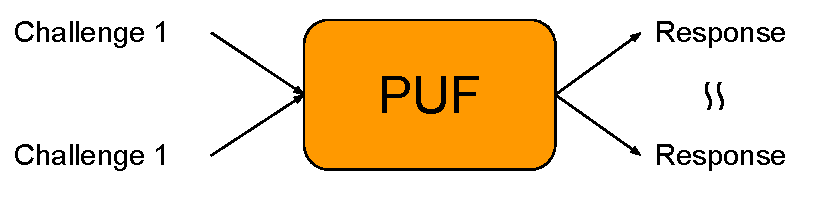
\includegraphics[width=0.75\textwidth]{images/reproducibility}
    \caption[reproducibility: responses to the same PUF challenge need to be similar]{reproducibility: responses to the same PUF challenge need to be similar~\cite{Kodytek2017}}
    \label{fig:reproducibility}
\end{figure}

\subsection*{Uniqueness}

While reproducibility talks about the behaviour of a specific \gls{puf}, uniqueness is defined with respect to a set of different \gls{puf} instances. Given the same challenge, two \glspl{puf} must produce a response that is different enough in the given metric. The metric used is the inter-Hamming distance (which will be defined later in Section~\ref{sec:uniqueness}).

\begin{figure}[ht!]
    \centering
    \captionsetup{justification=centering,margin=0.5cm}
    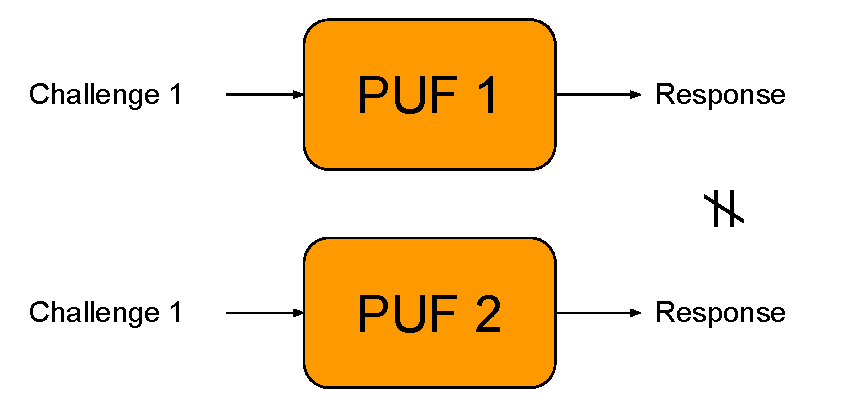
\includegraphics[width=0.75\textwidth]{images/uniqueness}
    \caption[uniqueness: two PUF instances must produce different responses if given the same challenge]{uniqueness: two PUF instances must produce different responses if given the same challenge~\cite{Kodytek2017}}
    \label{fig:uniqueness}
    % TODO cite
\end{figure}

\subsection*{Identifiability}\label{sec:identifiability}

Identifiability is tied to both uniqueness and reproducibility. Given a single challenge, if the responses from the same \gls{puf} are similar and responses from different \glspl{puf} are different enough, the responses can be used as a means of identification of each \gls{puf}. More formal characterization of the words `similar' and `different' as well as a concrete protocol for \gls{puf} identification is explained in Sections~\ref{sec:puf_evaluation} and~\ref{sec:identification}.

\subsection*{Physical unclonability}
 
Physical unclonability enforces that it is hard to break the uniqueness property. The `hardness' is expressed as a technical and physical infeasibility of creating two nearly identical \gls{puf} instances. In practice, even the manufacturer is unable to break uniqueness due to the uncontrollable physical laws on which the \gls{puf} implementation relies.

\subsection*{Unpredictability}

A \gls{puf} is said to be unpredictable, if given a limited set of challenge-response pairs, it is impossible to create an algorithm that predicts the remaining responses based on a challenge. This means that the challenge-response pair space is sufficiently random.

\subsection*{Mathematical unclonability}

While physical unclonability talks about the impossibility of creating a real-world clone of a specific \gls{puf}, mathematical unclonability requires that no algorithm can predict the \gls{puf} behaviour.

Mathematical unclonability is a stronger model of unpredictability. It assumes unlimited physical access to a specific \gls{puf} instance. The potential adversary can learn as many challenge-response pairs as he is capable of storing and can potentially make use of other \gls{puf} observations. Even in this situation, it should be impossible for the adversary to create a prediction algorithm capable of outputting a response based on a given challenge. 

Mathematical unclonability implies that the specific \gls{puf} implementation has a large number of possible challenges (more than the adversary could theoretically store). If this was not true, a simple lookup table of challenge-response pairs could be constructed, breaking mathematical unclonability. % TODO mention strong PUFs?

\subsection*{True unclonability}

\gls{puf} is considered truly unclonable if it is physically and mathematically unclonable. True unclonability thus implies mathematical and physical unclonability.

\subsection*{One-Wayness}

The one-wayness property is similar to the requirement of cryptographic one-way functions (for example hash functions). Given a \gls{puf} instance and a response, it should be impossible to create an inversion algorithm that can find a corresponding challenge to the response.

Similar to mathematical unclonability, the \gls{puf} needs to have a sufficiently large set of possible challenges and resulting responses in order to meet this property. Otherwise, it would be possible to construct a complete lookup table and find the wanted challenge.

\begin{figure}[h!]
    \centering
    \captionsetup{justification=centering,margin=0.5cm}
    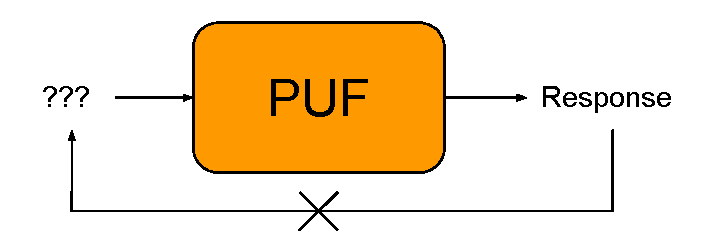
\includegraphics[width=0.75\textwidth]{images/one-wayness}
    \caption{one-wayness: it is impossible to find a challenge corresponding to a given response}
    \label{fig:one-wayness}
\end{figure}

\subsection*{Tamper Evidence}

Tampering with devices in order to compromise their integrity has proven to be a successful technique. For example, invasive attacks (such as microprobing) are able to extract sensitive data from the target system.\cite{Kommerling1999}

Tamper evidence helps to mitigate such attack vectors. The \gls{puf} must detect the attempt to tamper with the system and change its challenge-response pairs to a different set as if the \gls{puf} instance transforms itself to a completely different one.

To achieve this property, the \gls{puf} implementation needs to rely on physical properties that will necessarily change if the device is tampered with. This change will inherently transform the \gls{puf}.

%--------------------------------
\section{PUF classification}
%--------------------------------

A lot of different \gls{puf} implementations have been proposed. They can be classified based on fabrication, security and intrinsic evaluation\cite{Shital2017}\cite{McGrath2019}. A diagram of the discussed \gls{puf} classes is depicted in figure~\ref{fig:classification}.

\begin{figure}[ht!]
    \centering
    \captionsetup{justification=centering,margin=0.5cm}
    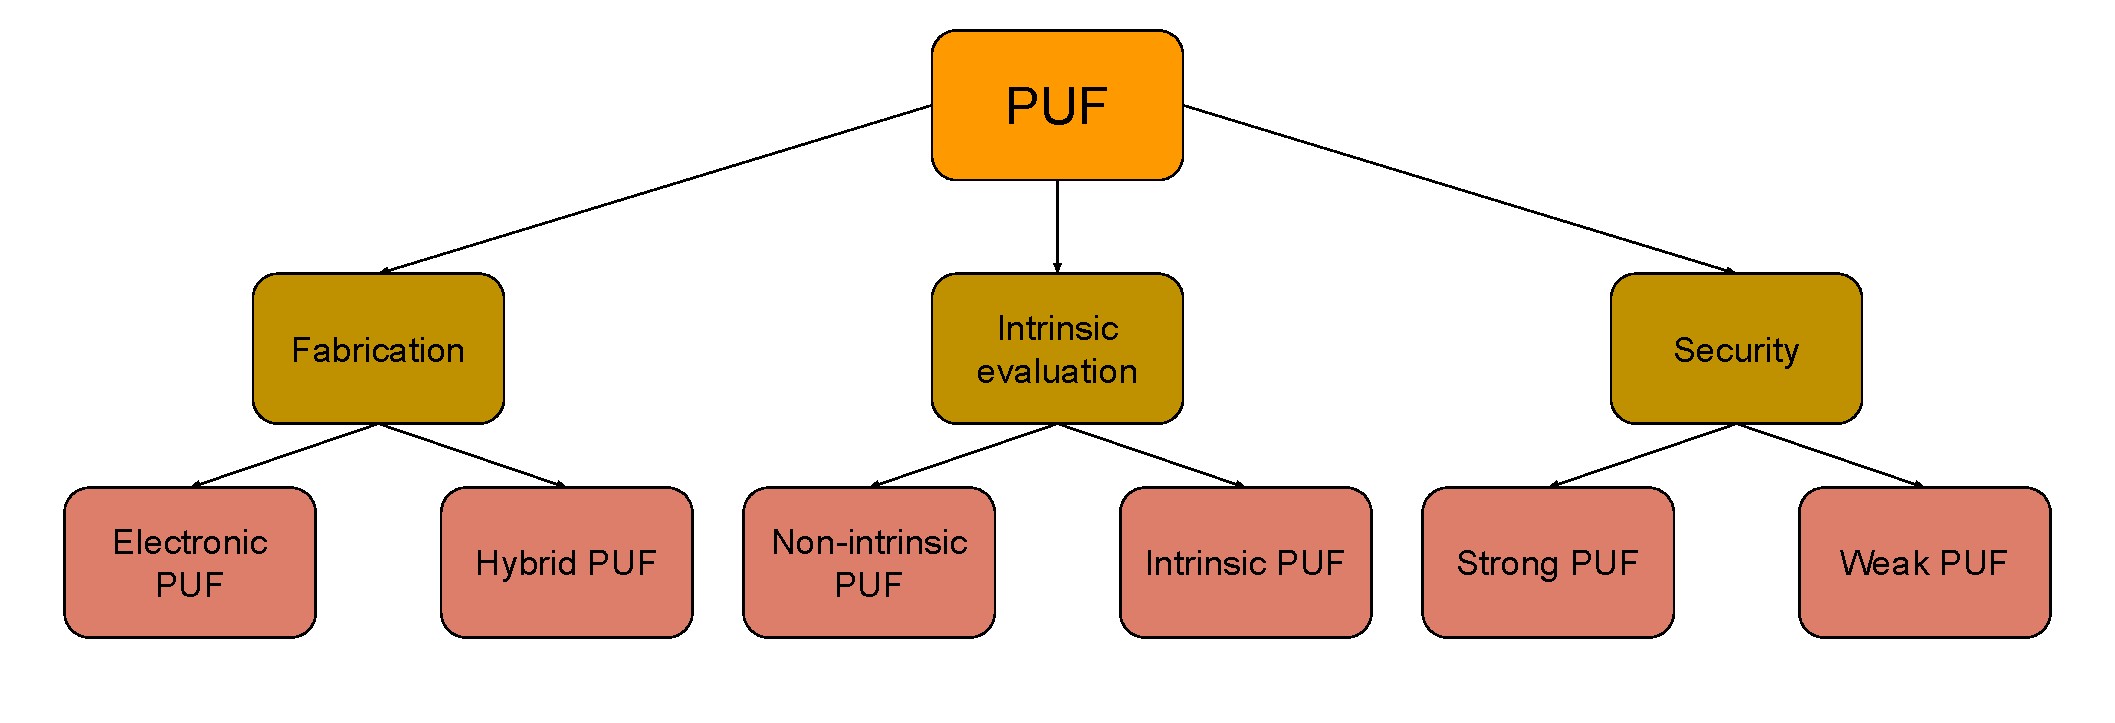
\includegraphics[width=\textwidth]{images/classification}
    \caption{classification of PUFs}
    \label{fig:classification}
\end{figure}

\subsection*{Electronic, silicon and hybrid PUFs}

Electronic \glspl{puf} source their randomness from electronic components. This means that they rely on properties such as capacitance, resistance or propagation delay of a circuit.

A large subclass of electronic \glspl{puf} is silicon \glspl{puf}. They can be constructed only using \gls{cmos} technology, therefore they can be implemented on the same die together with the main chip. This prevents the need to interface with additional circuitry using external buses, lowering cost and limiting the possibility of leaking sensitive data.\cite{Maes2013}

Examples of electronic \glspl{puf} are \gls{sram} \gls{puf}, \gls{ropuf} or arbiter \gls{puf}.

Hybrid \glspl{puf} use non-electronic phenomena to create their challenge-response pairs. While randomness introduced into the system is of non-electronic nature, the signal is usually processed and stored using electronic components. Hence the name hybrid \glspl{puf}. They can be based on optics (optical \gls{puf}), magnetism (magnetic \gls{puf}) or quantum effects (quantum \gls{puf}\cite{Koustubh2021}).


\subsection*{Intrinsic and non-intrinsic PUFs}

A \gls{puf} implementation is said to be intrinsic if it satisfies the following two conditions:

\begin{enumerate}
    \item responses are evaluated internally
    \item instance-specific random features are introduced implicitly during the manufacturing process
\end{enumerate}

Internal evaluation requires the measurement equipment of the \gls{puf} to be embedded in the device. This, similar to silicon \glspl{puf}, lowers cost and is more secure.

The second condition discusses the introduction of randomness into the system. Implicit randomness relies on process variations taking place during normal manufacturing, while explicit randomness needs to be created by special procedures which would have not been needed otherwise (such as doping with random dielectric particles for the construction of a coating \gls{puf}\cite{Kori2006}).

\gls{sram} and arbiter \glspl{puf} are examples of intrinsic \glspl{puf}. If the \gls{puf} construction does not satisfy the given properties, it is called non-intrinsic. For example, optical or coating \glspl{puf} are non-intrinsic.\cite{Maes2012}

\subsection*{Strong and weak PUFs}

Security based classification distinguishes \gls{puf} implementations according to the size of their challenge-response pair sets.

In order for a \gls{puf} to be classified as strong, its challenge-response pair set needs to be sufficiently large to prevent an exhaustive search by a possible attacker. The challenge-response pair size thus scales well (preferably exponentially) with some construction parameter.\cite{Guajardo2007}

On the other hand, weak \glspl{puf} have only a limited set of challenge-response pairs. Some \glspl{puf} can only have one pair. They are sometimes called \gls{pok}.

As the naming implies, strong \gls{puf} constructions possess, in some sense, greater security. Weak \glspl{puf} cannot be mathematically unclonable (and consequently cannot be truly unclonable or unpredictable). Strong \glspl{puf} can also be used in more applications, as explained in Section~\ref{sec:puf_applications}. However, it turns out that constructing a strong \gls{puf} is a very hard problem.\cite{Maes2013}

%--------------------------------
\section{PUF evaluation parameters}\label{sec:puf_evaluation}
%--------------------------------

As \glspl{puf} rely on uncontrollable physical processes to produce their responses, it is crucial to perform an analysis of their quality. Several evaluation parameters were defined by~\cite{Mispan2018},~\cite{Leest2010} and~\cite{Maiti2011} and they will be discussed here.

These parameters enable us to quantify the performance of \glspl{puf} and compare them. Some of them will be used to evaluate the \gls{sram} \gls{puf} implemented in this thesis in Sections~\ref{sec:rtc_evaluation} and~\ref{sec:deepsleep_evaluation}.

\noindent\newline
The following evaluation parameters will be defined:
\begin{itemize}
    \item Uniformity
    \item Reliability
    \item Uniqueness
    \item Bit-aliasing
    \item Randomness
\end{itemize}

Before the parameters can be defined, a notation used in the upcoming text is described here and in Table~\ref{table:notation} to avoid possible confusion.

The Hamming weight $\textrm{HW}(x)$ of a bit string \emph{x} is defined as the number of one bits in the string. 

The Hamming distance $\textrm{HD}(x, y)$ of two bit strings \emph{x} and \emph{y} is defined as a number of positions where the bits of \emph{x} and \emph{y} differ.

The reference response $R_{i}^{'}(n)$ is the expected response of \emph{n} bits produced by the chip \emph{i}. It is usually computed as a bitwise average between \emph{m} response samples taken in normal operating conditions. However, some works choose the reference response as the first measured sample.\cite{Kodytek2020}

\begin{table}[h!]
\centering
\begin{tabular}{c l} 
     Notation & Description\\
     \hline
     k & The number of devices\\ 
     m & The number of response samples\\
     n & The number of bits in a response\\ 
     $R_{i,j}(n)$ & The \emph{j}-th response (containing \emph{n} bits) of \emph{i}-th chip\\ 
     $R_{i}^{'}(n)$ & The reference response of \emph{i}-th chip, containing \emph{n} bits\\ 
     $r_{i,j}^{'}$ & The \emph{j}-th bit of a reference response of chip \emph{i}\\
     $\textrm{HW}(x)$ & The Hamming weight of \emph{x}\\
     $\textrm{HD}(x, y)$ & The Hamming distance between \emph{x} and \emph{y}\\
     \hline
    \end{tabular}
    \captionsetup{justification=centering,margin=0.5cm}
    \caption{Notation used in evaluation parameters definitions}
    \label{table:notation}
\end{table}

\subsection{Uniformity}\label{sec:uniformity}

Uniformity represents a proportion of zero and one states of the response bits. It is useful to determine if there exists a global bias towards any of these states. Since the \gls{puf} responses need to be unpredictable, there should not be any bias. Thus, the ideal value of uniformity is 50\%.

The uniformity property for one response of chip \emph{i} is defined by Equation~\ref{eq:uniformity}:

\begin{equation}\label{eq:uniformity}
    U_{i} = \frac{1}{n}\sum_{j=1}^{n}r_{i,j}^{'} = \frac{\textrm{HW}(R_{i}^{'}(n))}{n} \cdot 100\% 
\end{equation}

Uniformity can also be calculated as an average value between k \gls{puf} instances of the same type by Equation~\ref{eq:avg_uniformity}\cite{Maiti2011}:

\begin{equation}\label{eq:avg_uniformity}
    U_{\textrm{avg}} = \frac{1}{k}\sum_{i=1}^{k}U_{i} = \frac{1}{k}\sum_{i=1}^{k}\frac{\textrm{HW}(R_{i}^{'}(n))}{n} \cdot 100\%
\end{equation}

Since uniformity only measures a global proportion of the response bit states, it is not a perfect tool to detect a possible local bias. A trivial example could be a response defined in the following way:

\begin{equation}
    r_{i, j}^{'} =
    \begin{cases*}
        1 & if $j < \frac{m}{2}$ \\
        0 & otherwise
    \end{cases*}
\end{equation}

That is the first half of the response bits are ones and the second half are all zero bits. Uniformity $U_{i}$ for such a response is close to the ideal value of $50\%$ though the response is clearly not unpredictable.

\subsection{Reliability}\label{sec:reliability}

Reliability is a parameter that measures the consistency of \gls{puf} responses to the same challenge. It is tied to the reproducibility property from Section~\ref{sec:reproducibility}.

In order to calculate reliability, the intra-Hamming distance for a chip \emph{i} needs to be defined first\cite{Maiti2011}: 

\begin{equation}\label{eq:hd_intra}
    \textrm{HD-intra}_{i} = \frac{1}{m} \sum_{j=1}^{m}\frac{\textrm{HD}(R_{i,j}(n), R_{i}^{'}(n))}{n} \cdot 100 \%
\end{equation}

The reference $R_{i}^{'}(n)$ is obtained at nominal operating conditions (room temperature and normal voltage). The responses $R_{i, j}(n)$ are then taken at different conditions and the result is calculated. It essentially represents the percentage of bits that change compared to the reference response.

Reliability is then defined by Equation~\ref{eq:reliability}:

\begin{equation}\label{eq:reliability}
    \textrm{Reliability} = 100\% - \textrm{HD-intra}
\end{equation}

Since the reproducibility property requires \glspl{puf} to produce similar responses to the same challenge, the ideal $\textrm{HD-intra}_{i}$ value is $0\%$ and thus reliability needs to be close to $100\%$.

\subsection{Uniqueness}\label{sec:uniqueness}

Uniqueness measures how much responses from different \glspl{puf} vary. It is estimated by the inter-Hamming distance defined by Equation~\ref{eq:uniqueness}:

\begin{equation}\label{eq:uniqueness}
    \textrm{HD-inter} = \frac{2}{k(k-1)}\sum_{i=i}^{k-1} \sum_{j=i+1}^{k} \frac{\textrm{HD}(R_{i}^{'}(n),R_{j}^{'}(n))}{n} \cdot 100\%
\end{equation}

The original definition of $\textrm{HD-inter}$ by~\cite{Maiti2010} does not specify how to choose the responses to calculate the Hamming distance from. However,~\cite{Kodytek2020} uses the reference responses and this definition will be used in future calculations in this thesis.

The inter-Hamming distance takes all combinations of pairs of devices and computes the average Hamming distance of their responses. The uniqueness property of \glspl{puf} in Section~\ref{sec:properties} requires that the responses should differ as much as possible. This is achieved when $\textrm{HD-inter}$ is close to its ideal value of $50\%$.

\subsection{Bit-aliasing}\label{sec:bit_aliasing}

Uniformity in Section~\ref{sec:uniformity} looks at the global bias of \gls{puf} responses from a single device. On the other hand, bit-aliasing measures the proportion of zero and one state of a single bit across different devices.

Bit-aliasing is calculated as the percentage Hamming weight of the \emph{j}-th bit. It is defined by Equation~\ref{eq:bit_aliasing}\cite{Maiti2011}:

\begin{equation}\label{eq:bit_aliasing}
    \textrm{Bit-aliasing}_{j} = \frac{1}{k}\sum_{i=1}^{k}r_{i, j}^{'} \cdot 100\%
\end{equation}

Same as for uniformity, the ideal value for bit-aliasing is $50\%$. Values close to 0 or 100\% would indicate bits that stay the same across different \gls{puf} instances, violating the uniqueness property.

\subsection{Randomness}

As \gls{puf} responses need to be unpredictable, they are required to contain sufficient entropy. According to~\cite{Leest2010}, there are several ways to test whether the response data is sufficiently random. Two are described here, the compression test and the \acrshort{nist} randomness test.

\subsubsection*{NIST randomness test}

The \acrshort{nist} randomness test uses the \acrshort{nist} statistical test suite to determine if the data is sufficiently random. Each test from the battery is tested for the null hypothesis that the response data is truly random on some set significance level.

Furthermore, each test is executed multiple times on different sequences of the data and a p-value for each run is calculated. These p-values are then tested for the null hypothesis that they are from a uniform distribution, as would be the case for truly random data.\cite{NIST2010}

However, not all tests can be used as they require more input data than is practically possible to generate by the \gls{puf}. Tests for which only 170-bit string suffices are listed here\cite{Leest2010}:

\begin{itemize}
    \item Frequency (monobit) test
    \item Frequency test within a block
    \item Runs test
    \item Test for longest run of ones in block
    \item Serial test
    \item Approximate entropy test
    \item Cumulative sums (Cusum) test
\end{itemize}

\subsubsection*{Compression test}

The idea behind compression test is simple. If a lossless compression algorithm is able to reduce the size of the tested data, it does not have full entropy\footnote{Meaning the entropy in bits is the same as the length of the data in bits.}\cite{Leest2010}.

A good example of a compression algorithm to use is the \gls{ctw} algorithm as it was shown to produce the best results out of the commonly used entropy estimators\cite{Yun2008}.

\section{PUF applications}\label{sec:puf_applications}
%--------------------------------

Thanks to the properties described in Section~\ref{sec:properties}, \glspl{puf} are suitable for several cryptographic applications. Three main uses of \glspl{puf} according to~\cite{Maes2012} will be described here: identification, authentication and cryptographic key generation.


\subsection{Identification}\label{sec:identification}

A \gls{puf} can be compared to a device's fingerprint. The \gls{puf} provides an inherent identifying feature\footnote{Inherent identity is a unique characteristic of the device itself (a \gls{puf} response), while assigned identity is an artificially made up property (a serial number).} to the entity encapsulating it.  Therefore, device identification is a natural application for \glspl{puf}. A simple identification protocol using the device's \gls{puf} is described.

The process of device identification consist of two phases: enrollment and identification\cite{Maes2012}.

\begin{description}
    \item[Enrollment phase:] \hfill \\ In this phase, the inherent identifying feature of every considered device is collected. This means saving a \gls{puf} response from each device to a database.
    \item[Identification phase:] \hfill \\ When the device needs to be identified, it generates its \gls{puf} response. The response is then compared to other responses stored in the database.
\end{description}

However, the comparison of the presented \gls{puf} response is not straightforward. Since the \gls{puf} relies on physical state of the system, errors can arise while generating responses. For this reason, comparison is based on the \gls{hd} rather than on equality.

The property of identifiability (discussed in Section~\ref{sec:identifiability}) tells us that responses from a specific device will be similar (have low \gls{hd}) and responses from different devices will be far apart (have high \gls{hd}). Thus, a threshold value of \gls{hd} needs to be chosen. Responses with lower \gls{hd} than the threshold will be considered to have originated from the same device.

\begin{figure}[ht!]
    \centering
    \captionsetup{justification=centering,margin=0.5cm}
    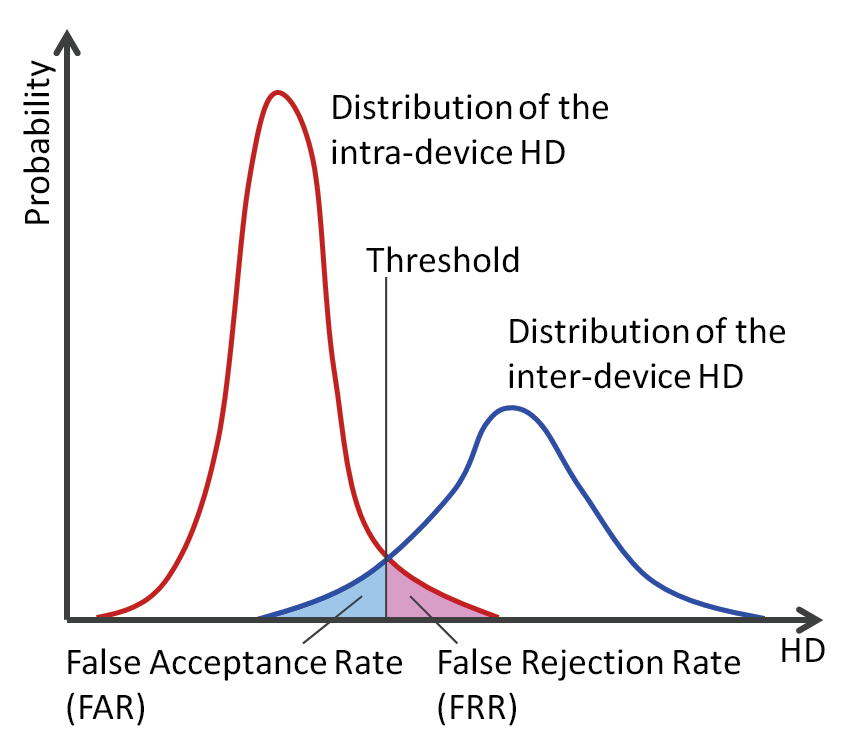
\includegraphics[scale=0.25]{images/identification_histogram.png}
    \caption[PUF identification: intra and inter HD distributions]{PUF identification: intra and inter HD distributions\cite{Hori2013}}
    \label{fig:puf_inter_intra_hd}
\end{figure}

The threshold can be chosen based on the distributions of inter and intra \glspl{hd}. While the inter-\gls{hd} is a measure of how responses from different devices differ, the intra-\gls{hd} indicates the similarity of responses from the same device.

If the distributions of inter and intra \glspl{hd} do not overlap, threshold value between the distributions is optimal. The \gls{far} (a probability of falsely identifying a device) and \gls{frr} (the probability of falsely rejecting a device) are zero.

If the distributions overlap, a compromise between \gls{far} and \gls{frr} must be made. Reducing \gls{far} will inevitably increase \gls{frr} and vice versa. Figure~\ref{fig:puf_inter_intra_hd} illustrates a possible intra and inter \gls{hd} distributions and a chosen threshold.

\subsection{Authentication}

Authentication requires the entity, which wants to authenticate itself to a verifier, to provide a proof of its identity. The entity also needs to convince the verifier that it actively participated in the creation of the proof.\cite{Maes2012}

A simple protocol based on the challenge-response pairs of \glspl{puf} will be presented here. It is divided into two distinct phases: enrollment and authentication.\cite{Devadas2008}

\begin{description}
    \item[Enrollment phase:] \hfill \\ During this phase, a trusted third party (the verifier) is in possession of the device which will later be authenticated. A sufficient number of randomly generated challenges along with the corresponding responses (obtained from the device) is saved to a database.
    \item[Authentication phase:] \hfill \\ When the device needs to be authenticated, the verifier chooses a challenge from the database and sends it to the device. The device then responds with the corresponding response. Finally, the obtained and the previously recorded responses are compared. If they are sufficiently similar, the device is authenticated successfully. This challenge-response pair is then deleted from the database and never used again.
\end{description}

The whole process of this \gls{puf}-based authentication protocol is illustrated in Figure~\ref{fig:authentication_process}.

\begin{figure}[ht!]
    \centering
    \captionsetup{justification=centering,margin=0.5cm}
    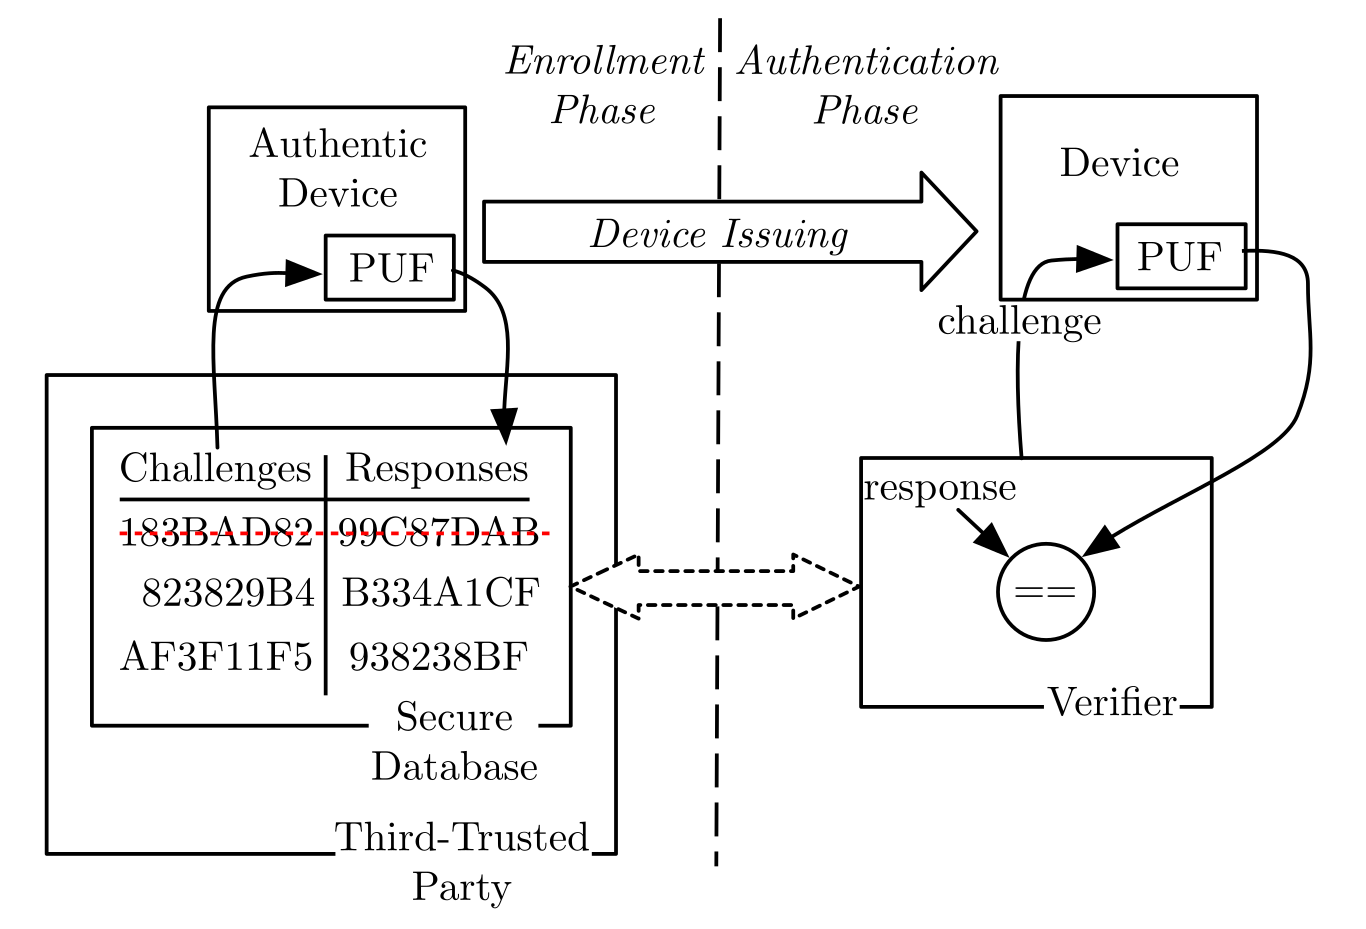
\includegraphics[width=0.7\textwidth]{images/authentication_process.png}
    \caption[PUF-based authentication protocol]{PUF-based authentication protocol\cite{Barbareschi2018}}
    \label{fig:authentication_process}
\end{figure}

The comparison of the responses is done in the same way as in \gls{puf}-based identification (Section~\ref{sec:identification}). The \gls{hd} is used as a distance metric and a threshold for accepting the response must be chosen appropriately.

The challenge-response pairs are deleted from the database and never reused to prevent a potential man-in-the-middle attack. Since this is not a threat, the communication between the device and the verifier does not need to be secured.

This protocol is simple and has its drawbacks. It only provides a limited number of authentications for the verifier given by the number of stored challenge-response pairs. The authentication is only one-way, the verifier is never authenticated to the device. It requires the \gls{puf} to be strong (to have a large number of available challenge-response pairs).

More advanced \gls{puf}-based authentication protocols that address some of the aforementioned drawbacks have been developed by~\cite{Maes2013},~\cite{Barbareschi2018} and~\cite{Rostami2014}.

\subsection{Key generation}

Keys are required in the majority of cryptographic applications. They need to contain true randomness in order to be unpredictable and unique. The cryptographic key then needs to be stored and retrieved securely. These conditions are hard to meet and a myriad of cryptographic systems have been broken because of bad generation or handling of keys.\cite{Maes2012_2}

\gls{puf}-based cryptographic key generation tries to solve those problems. The key is not stored in any memory and is generated by the \gls{puf} on demand. In some way, it is imprinted in the \gls{puf} itself. Furthermore, the uniqueness and unpredictability property of \glspl{puf}, which arise from their uncontrollable physical properties, introduce the necessary randomness.

Since the \gls{puf} responses are noisy and not 100\% reliable, care needs to be taken while generating cryptographic keys. The keys need to be the same every time, otherwise the cryptographic algorithms using it would not produce the desired output. For this reason, \glspl{ecc} are used to obtain the same key every time with sufficient probability.

\begin{figure}[h!]
    \centering
    \captionsetup{justification=centering,margin=0.5cm}
    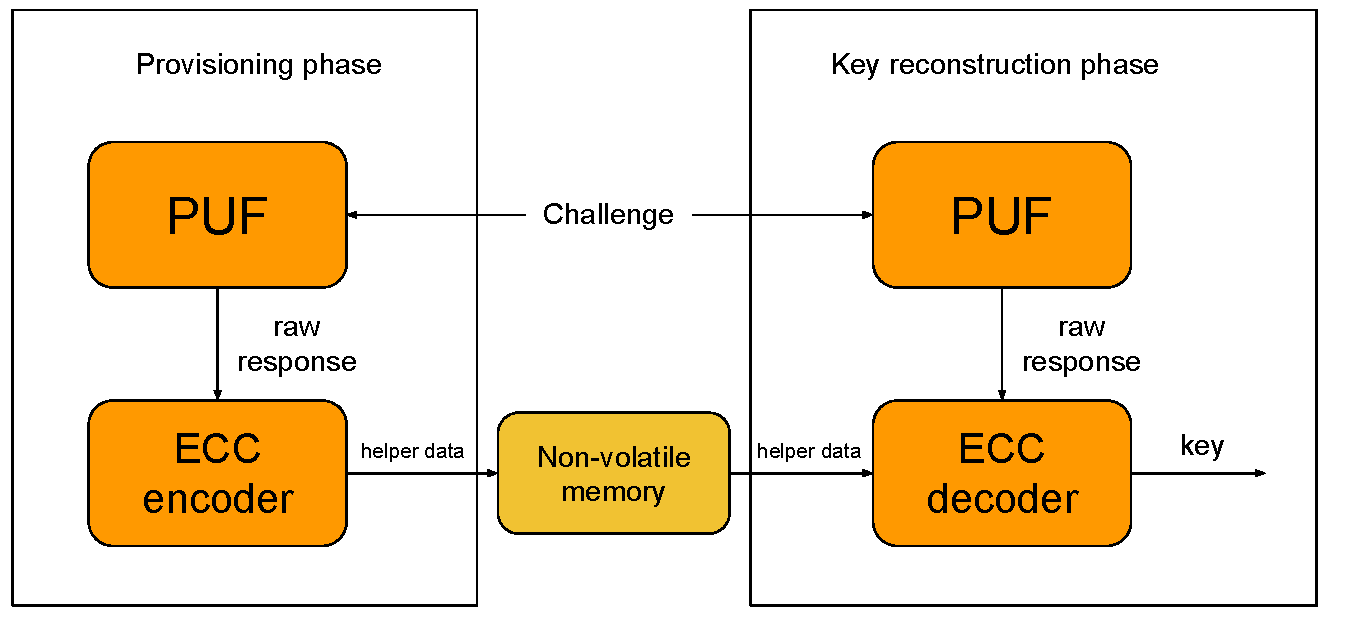
\includegraphics[width=\textwidth]{images/key_generation.pdf}
    \caption[PUF-based key-generation mechanism]{PUF-based key-generation mechanism, inspired by~\cite{Gao2017}}
    \label{fig:key_generation}
\end{figure}

The process of \gls{puf}-based key generation is divided into two phases: enrollment and key reconstruction\cite{Mispan2018}. It is illustrated in Figure~\ref{fig:key_generation}.

\begin{description}
    \item[Enrollment phase:] \hfill \\ In this phase, \gls{puf} responses are generated and processed by the \gls{ecc} algorithm to construct the cryptographic key. The \gls{ecc} calculates helper data from the key and saves it to a non-volatile memory. This data will later be used to reconstruct the key. The helper data can also contain a \gls{puf} configuration.
    \item[Key regeneration phase:] \hfill \\ When the key is needed, the \gls{puf} produces a response and feeds it to the \gls{ecc} algorithm. The key is then reconstructed by the \gls{ecc} using the response and the corresponding helper data saved in the non-volatile memory.
\end{description}

The \gls{ecc} used is usually a simple repetition code or a \gls{bch} code. However, any \gls{ecc} can be used and the codes can even be concatenated in order to increase efficiency.\cite{Bosch2008}

After key regeneration, a raw bit string key is obtained. It can be used immediately with some cryptosystems (typically symmetric ciphers such as AES). However, some systems put restrictions on the key (RSA needs two prime numbers), thus requiring further processing. % TODO kde jsem ztratil zdroj?

Key generation is a typical application of weak \glspl{puf}\cite{Herder2014}. As the \gls{sram} \gls{puf} implemented in this thesis is classified as weak, a simple key generation algorithm will be tested on top of the \gls{puf}.

It is even possible for a weak \gls{puf} to provide authentication without the need for a large number challenge-response pairs. Once the key is generated by the weak \gls{puf}, it can be used in other cryptographic algorithms which provide authentication such as \gls{mac} or digital signatures (at the cost of additional hardware/software).\cite{Herder2014}


% TODO hash po rekonstrukci klice? (zdroj FPGA Intrinsic PUFs and Their Use for IP Protection jako privacy amplification)

%--------------------------------
\section{PUF implementations}
%--------------------------------

\subsection{Optical PUF}\label{sec:optical_puf}
\subsection{SRAM PUF}
\subsubsection*{SRAM PUF and its properties}\label{sec:srampuf_properties}
% TODO mozna neco o SRAM aging? (intrinsicID meli nejaky whitepaper)

%---------------------------------------------------------------
\chapter{ESP32 platform}
%---------------------------------------------------------------

%---------------------------------------------------------------
\chapter{SRAM PUF implementation on ESP32}
%---------------------------------------------------------------

%--------------------------------
\section{RTC SRAM based PUF}
%--------------------------------

\subsection{RTC SRAM power control}
\subsection{SRAM analysis based on temperature and power off time}
\subsection{PUF evaluation parameters}\label{sec:rtc_evaluation}

%--------------------------------
\section{Deep sleep based PUF}
%--------------------------------

\subsection{Deep sleep SRAM power control}
\subsection{SRAM analysis based on temperature and power off time}
\subsection{PUF evaluation parameters}\label{sec:deepsleep_evaluation}

%--------------------------------
\section{?PUF response data image} % TODO how to name this section?
%--------------------------------

%---------------------------------------------------------------
\chapter{Reliable PUF response extraction} % TODO should this be its own section or part of the previous one?
%---------------------------------------------------------------

%--------------------------------
\section{Stable bits selection}
%--------------------------------

%--------------------------------
\section{Error correction code}
%--------------------------------

%--------------------------------
\section{Provisioning}
%--------------------------------

%--------------------------------
\section{Combining power control methods}
%--------------------------------

%--------------------------------
\section{Reliability testing}
%--------------------------------

%---------------------------------------------------------------
\chapter{ESP32 SRAM PUF library}
%---------------------------------------------------------------

%---------------------------------------------------------------
\chapter{Conclusion}
%---------------------------------------------------------------

